\section{Úvod}
V práci je nejprve popsána struktura řídících smyček pohybu lékařského CT manipulátoru Phillips Azurion 7 C20
včetně proudové kalibrační tabulky (CCT). Kalibrační tabulka hraje zásadní roli pro dosažení přesných pohybů jednotlivých kloubů a~zajištění přesného a~konzistentního chování při lékařských zákrocích. Z~důvodu přirozeného opotřebení stroje je však nutná pravidelná rekalibrace, která vede k~nežádoucím odstávkám. Cílem této práce je proto navrhnout řešení, jak minimalizovat potřebu rekurentních manuálních rekalibrací stroje pomocí vhodného algoritmu aktualizace CCT, čímž by se zvýšila přesnost a~spolehlivost manipulátoru a~také snížil počet odstávek stroje.
\par
Tato práce se zabývá řešením pomocí B-spline interpolace/aproximace. Interpolace a~aproximace jsou rozhodujícími technikami pro problém aktualizace CCT, které umožňují vyvodit správné hodnoty v~bodech ležících mimo síť naměřených bodů v~této tabulce.\par
% Navrhované řešení by mohlo výrazně zlepšit proces kalibrace, což by v~konečném důsledku vedlo ke spolehlivějšímu a 
Text je rozdělen na několik hlavních částí:
\begin{enumerate}
    \item \nameref{section: řízený a~říddící systém} --- část zaměřená na řízený a~řídící systém, která obsahuje technické specifikace robota, popis problému a~také zvolený přístup řešení
    \item \nameref{section: NURBS teorie} --- obsáhlá kapitola, ve které je rozebrána veškerá teorie k~NURBS křivkám/povrchům včetně kompletně vlastní implementace v~Matlabu dle knihy \cite{The_NURBS_Book}. Kapitola obsahuje ukázky výsledků jednotlivých algoritmů na obecných datech.
    \item \nameref{section: návrh automatické kalibraci} --- část, ve které jsou vizualizovány výsledky aplikace principů NURBS teorie na reálných datech. Dále v~této kapitole byly také využity techniky z~oblasti zpracování signálů, za účelem nalezení vhodných částí měření, které by se daly využít pro aktualizaci CCT.
\end{enumerate}
Všechny hodnoty poloh a~proudů pro jednotlivé klouby byly v~práci znormovány tak, aby bylo omezeno riziko úniku citlivých dat společnosti Phillips. Jedná se tak o~bezrozměrné veličiny, u~kterých nejsou uvedeny jednotky.
\par
V~případě ukázky animací je zobrazeno pouze 6 snímků pro tištěnou verzi, plná verze animace je obsažena v~příloze či v~digitální verzi dokumentace. Celá tato práce včetně zdrojového kódu je veřejně dostupná online --- \cite{Github}.
% \begin{imagepage}
% https://www.philips.cz/healthcare/product/HCNCVD207/azurion-7-c20-with-flexarm-image-guided-therapy-system
% https://www.philips.de/c-dam/corporate/newscenter/de/press-releases/2019/20190122-azurion-7-c20-mit-flexarm/philips-azurion-7-c20-mit-flexarm-produkt2-un-hs-20190122.download.jpg
\begin{figure}[H]
    \centering
    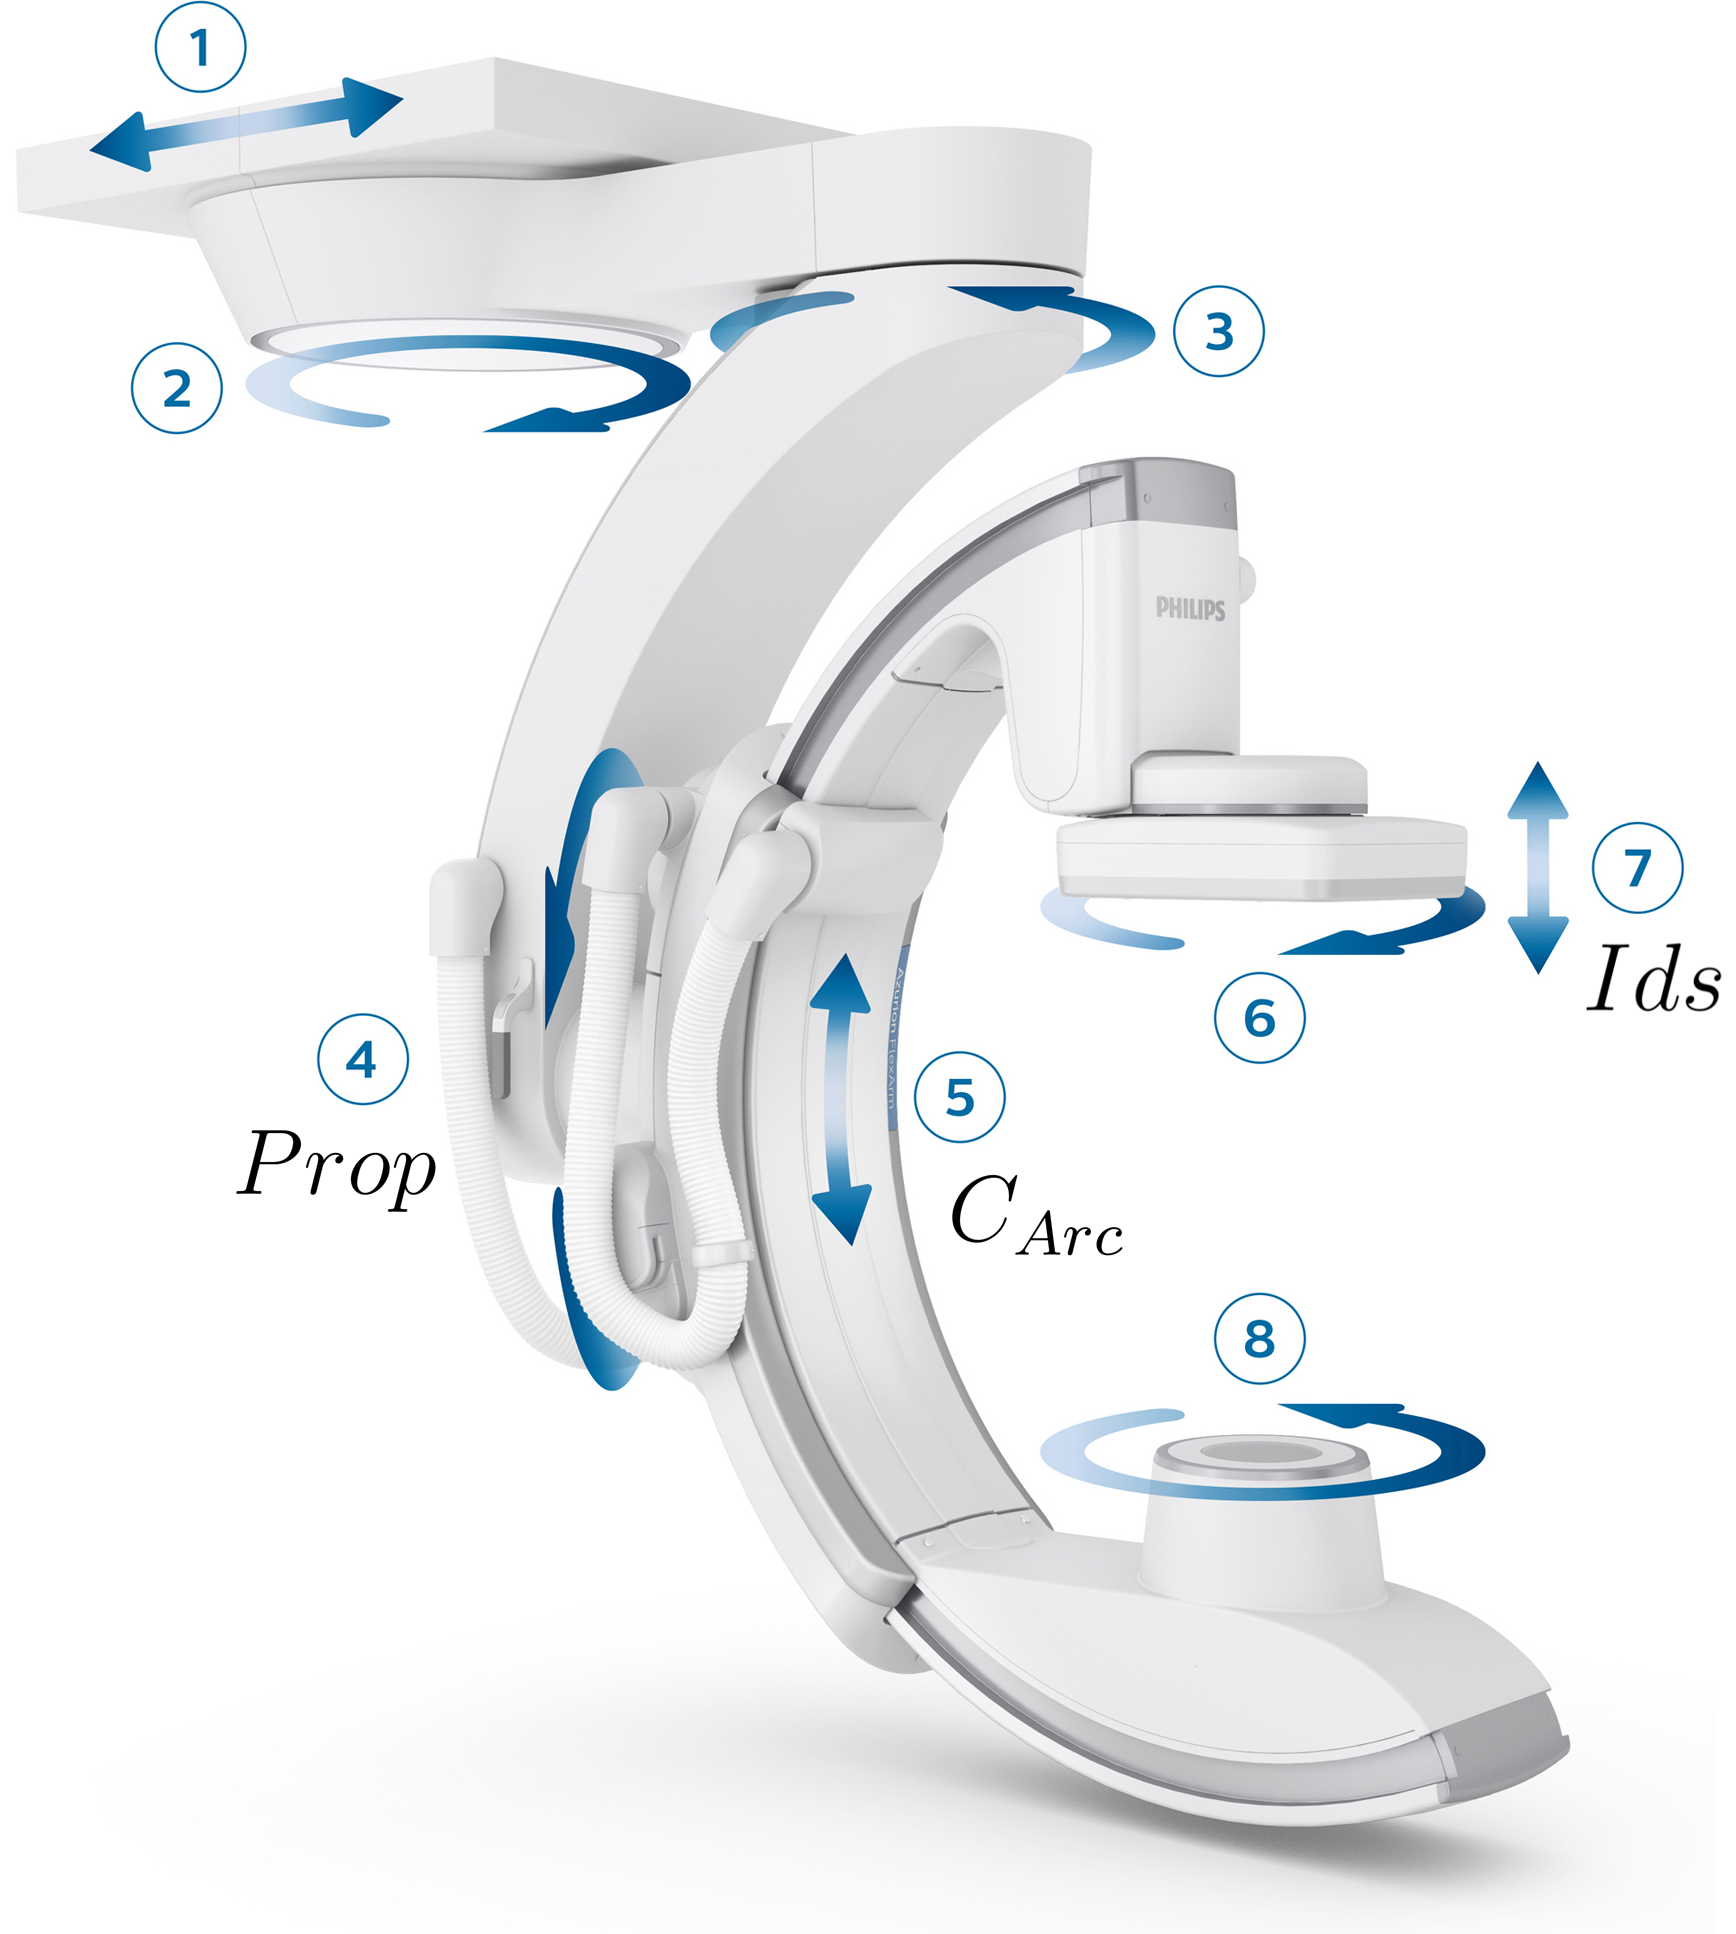
\includegraphics[width=\textwidth]{Img/Azurion 7 C20 with FlexArm modified.png}
    \caption[Výpočetní tomograf s~8 stupni volnosti Phillips Azurion 7 C20]{Výpočetní tomograf s~8 stupni volnosti Phillips Azurion 7 C20 --- \cite{Azurion}}
    \label{fig:Výpočetní tomograf}
\end{figure}
% \end{imagepage}